\section{Linux Kernel}
\subsection{Kernel编译}
\subsubsection{安装必要的软件包}
\begin{code-block}{bash}
yum install ncurses-devel bison flex elfutils-libelf-devel bc openssl-devel -y
\end{code-block}

\subsubsection{设置编译选项}
\begin{code-block}{bash}
make menuconfig
\end{code-block}

\subsubsection{编译内核}
\begin{code-block}{bash}
make
# 如果是在多核服务器上进行编译,可以增加编译参数,提高编译速度
# make -j32 #32表示cpu的核数
\end{code-block}

\subsubsection{安装内核模块}
\begin{code-block}{bash}
make modules_install
\end{code-block}

安装内核模块的操作,会将编译生成的内核模块复制到/lib/modules/\{kernel-version\}/下。

\subsubsection{安装内核}
\begin{code-block}{bash}
make install
\end{code-block}

安装内核的过程主要完成了以下的工作:将编译内核时生成的内核镜像bzImage拷贝到/boot目录下,
并将这个镜像命名为vmlinuz-\{kernel-version\}。如果使用x86的cpu,则该镜像位于arch/x86/boot/目录下;
将目录下的System.map拷贝到/boot/目录下,重新命名为System.map-\{kernel-version\},该文件中存放了内核的符号表。
将目录下的.config拷贝到/boot/目录下,重新命名为config-\{kernel-version\}

\subsubsection{创建initrd.img文件}
\begin{code-block}{bash}
mkinitrd  /boot/initrd.img-{kernel-version} {kernel-version}
\end{code-block}

initrd.img即为初始化的ramdisk文件,它是一个镜像文件。

\subsubsection{修改grub}
\begin{code-block}{bash}
grub2-mkconfig -o /boot/grub2/grub.cfg
\end{code-block}

修改完成之后,重启服务器,即可发现新编译的内核,如下图:
图 \nameref{fig:new-kernel}
\begin{figure}[H]
  \centering
  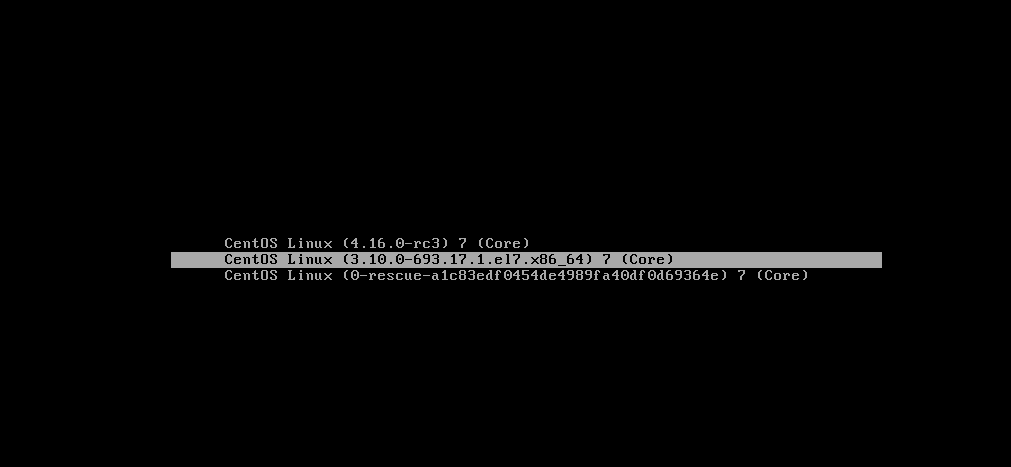
\includegraphics[scale=0.6]{new-kernel.png}
  \caption{新编译内核 \protect\footnotemark}
  \label{fig:new-kernel}
\end{figure}

\subsection{编写自己的内核模块}
在编写自己的内核模块的时候,一般需要2个文件:一个c代码文件,包含了自己的内核模块
内在逻辑实现;一个makefile文件,用于编译自己的内核模块。以最简单的hello world为例。
C代码如下:
\begin{code-block}{c}
// hello_kernel.c
#include <linux/init.h>
#include <linux/module.h>
#include <linux/kernel.h>

// 必须,标明模块的许可声明
MODULE_LICENSE("GPL");

// 模块的加载函数,即加载该模块之后,执行的操作
static int hello_init(void)
{
    printk(KERN_ALERT "hello,I am zhangjl\n");
    return 0;
}

// 模块的卸载函数,即该模块卸载之后,应当执行什么操作
static void hello_exit(void)
{
    printk(KERN_ALERT "goodbye,kernel\n");
}

// 注册模块对应的操作
module_init(hello_init);
module_exit(hello_exit);

// 可选,表示该模块的作者和其他信息
MODULE_AUTHOR("zhangjl");
MODULE_DESCRIPTION("This is a simple example!\n");
MODULE_ALIAS("A simplest example");
\end{code-block}

Makefile文件内容如下:
\begin{code-block}{make}
obj-m += hello_kernel.o
#generate the path
CURRENT_PATH:=$(shell pwd)
#the current kernel version number
LINUX_KERNEL:=$(shell uname -r)
#the absolute path
LINUX_KERNEL_PATH:=/usr/src/kernels/$(LINUX_KERNEL)
#complie object
all:
        make -C $(LINUX_KERNEL_PATH) M=$(CURRENT_PATH) modules
#clean
clean:
        make -C $(LINUX_KERNEL_PATH) M=$(CURRENT_PATH) clean
\end{code-block}

然后执行make。执行完毕之后,会在当前目录生成hello\_kernel.ko,这个文件即是我们
所需要的内核模块。执行insmod hello\_kernel.ko,在/var/log/message当中,会发现有hello的输出,执行
rmmod hello\_kernel,在/var/log/message当中,会发现有goodbyd的输出。整个简单的模块
就算完成了。

\subsection{Linux的进程遍历}
一个进程是由进程控制块(PCB),代码段和数据段组成的;并且,OS通常是通过PCB来感知
一个进程的存在。其实PCB就是操作系统对每个进程的代码描述。linux内核中使用task\_struct
结构来描述一个PCB(具体可以在linux/kernel/sched.c查看源码);多个进程则常常使用双链表
等来进行组织。比如可运行状态的进程组成可运行队列,等待状态的进程组成等待队列等。

list\_head为linux内核当中常用的数据结构,用于构造双链表,关于list\_head的具体用法,可以
参见c部分的宏定义高级使用部分。而task\_struct的定义类似于如下的代码:
\begin{code-block}{c}
struct task_struct {
        struct thread_info    thread_info;
        struct list_head      tasks;
};
\end{code-block}

由于该结构体当中存在list\_head的变量,因此,我们可以利用该变量来访问整个task\_strut,
进而获取我们需要的信息。完整代码如下:
\begin{code-block}{c}
#include <linux/init.h>
#include <linux/module.h>
#include <linux/kernel.h>
#include <linux/sched.h>
#include <linux/sem.h>
#include <linux/list.h>

MODULE_LICENSE("GPL");
static int hello_init(void)
{
        printk(KERN_ALERT "hello,I am zhangjl\n");
        return 0;
}

static int traverse_init(void)
{
       struct task_struct *pos;
       struct list_head *current_head;
       int count=0;
       printk("Traversal module is working..\n");
       current_head=&(current->tasks);
       list_for_each_entry(pos,current_head,tasks)
       {
              count++;
              printk("[process %d]: %s\'s pid is %d\n",count,pos->comm,pos->pid);
       }
       printk(KERN_ALERT"The number of process is:%d\n",count);
       return 0;
}

static void hello_exit(void)
{
    printk(KERN_ALERT "goodbye,kernel\n");
    traverse_init();
}

module_init(hello_init);
module_exit(hello_exit);
MODULE_AUTHOR("zhangjl");
MODULE_DESCRIPTION("This is a simple example!\n");
MODULE_ALIAS("A simplest example");

\end{code-block}

其中,current是一个宏,即为系统内正在运行的进程。编译该文件,然后加载该模块,在
系统日志当中,即可发现对应的输出。

\subsection{Linux的进程间通信(IPC)}
Linux常见的进程间通信模式主要如下:
\begin{itemize}
    \item 管道pipe

            管道是一种半双工的通信方式,数据只能单向流动,而且只能在具有亲缘关系的进程间使用。进程的亲缘关系通常是指父子进程关系。
    \item 命名管道FIFO

            有名管道也是半双工的通信方式,但是它允许无亲缘关系进程间的通信。
    \item 消息队列MessageQueue

            消息队列是由消息的链表,存放在内核中并由消息队列标识符标识。消息队列克服了信号传递信息少、管道只能承载无格式字节流以及缓冲区大小受限等缺点。
    \item 共享存储SharedMemory

            共享内存就是映射一段能被其他进程所访问的内存,这段共享内存由一个进程创建,但多个进程都可以访问。共享内存是最快的 IPC 方式,它是针对其他进程间通信方式运行效率低而专门设计的。它往往与其他通信机制,如信号两,配合使用,来实现进程间的同步和通信。
    \item 信号量Semaphore

            信号量是一个计数器,可以用来控制多个进程对共享资源的访问。它常作为一种锁机制,防止某进程正在访问共享资源时,其他进程也访问该资源。因此,主要作为进程间以及同一进程内不同线程之间的同步手段。
    \item 套接字Socket

            套解口也是一种进程间通信机制,与其他通信机制不同的是,它可用于不同及其间的进程通信。
    \item 信号 ( sinal )

            信号是一种比较复杂的通信方式,用于通知接收进程某个事件已经发生。
\end{itemize}

\subsubsection{管道方式}
管道,通常指无名管道,是 UNIX 系统IPC最古老的形式。
\begin{itemize}
    \item 半双工

            数据只能在一个方向上流动,具有固定的读端和写端。
    \item 亲缘关系

            只能用于具有亲缘关系的进程之间的通信(也是父子进程或者兄弟进程之间)。
    \item 特殊文件

            对于它的读写也可以使用普通的read、write 等函数。但是它不是普通的文件,并不属于其他任何文件系统,并且只存在于内存中。
\end{itemize}

当一个管道建立时,它会创建两个文件描述符:fd[0]为读而打开,fd[1]为写而打开。如下图:\nameref{fig:pipe}
\begin{figure}[H]
  \centering
  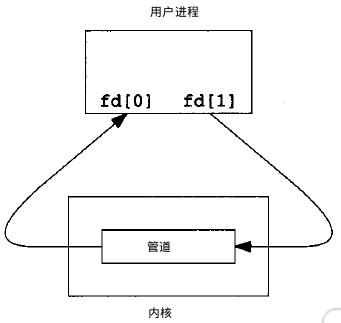
\includegraphics[scale=0.8]{pipe.png}
  \caption{管道}
  \label{fig:pipe}
\end{figure}
需要注意的是,fd[0]永远用于读取,不管是子进程还是父进程,都只能从fd[0]读取;fd[1]永远用于写入,子进程和父进程都只能从
fd[1]写入。如果fd的使用搞反,则会导致消息无法正常传递。

单个进程中的管道几乎没有任何用处。所以,通常调用 pipe 的进程接着调用 fork,这样就创建了父进程与子进程之间的 IPC 通道。如下图所示:\nameref{fig:fork_pipe}
\begin{figure}[H]
  \centering
  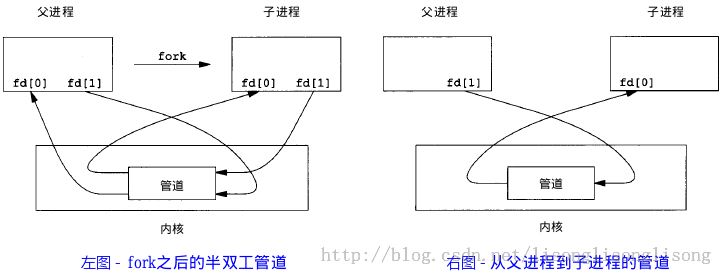
\includegraphics[scale=0.6]{fork_pipe.png}
  \caption{fork管道}
  \label{fig:fork_pipe}
\end{figure}

使用管道的具体方式如下:
\begin{code-block}{c}
#include <stdio.h>
#include <unistd.h>

int main(int argc, char * argv[])
{
        int fd[2];
        pid_t pid;
        char buf[20];

        if(0 > pipe(fd))
        {
                printf("Create Pipe Error!\n");
                return -1;
        }
        if(0 > (pid = fork()))
        {
                printf("Fork error\n");
                return -1;
        }
        if(0 == pid)
        {
#if 1
                // 父进程接收
                close(fd[1]);
                read(fd[0], buf, 20);
                printf("%s in pid %d\n", buf, pid);
                close(fd[0]);
#else
                // 父进程输入
                printf("pid: %d\n", pid);
                close(fd[0]);
                write(fd[1], "Hello World\n", 12);
                close(fd[1]);
#endif
        }
        else{
#if 1
                // 子进程输入
                printf("pid: %d\n", pid);
                close(fd[0]);
                write(fd[1], "Hello World\n", 12);
                close(fd[1]);
#else
                // 子进程接收
                close(fd[1]);
                read(fd[0], buf, 20);
                printf("%s in pid %d\n", buf, pid);
                close(fd[0]);
#endif
        }
        return 0;
}
\end{code-block}

\subsubsection{命名管道FIFO}
FIFO,也称为命名管道,它是一种文件类型。FIFO可以在无关的进程之间交换数据,与无名管道不同。FIFO有路径名与之相关联,它以一种特殊设备文件形式存在于文件系统中。
通常使用mkfifo创建一个命名管道。一旦创建了一个 FIFO,就可以用一般的文件I/O函数操作它。FIFO的通信方式类似于在进程中使用文件来传输数据,只不过FIFO类型文件同时具有管道的特性。
在数据读出时,FIFO管道中同时清除数据,并且“先进先出”。
下面的例子演示了使用 FIFO 进行 IPC 的过程。
Server端负责创建fifo,并保持监听。
\begin{code-block}{c}
// server.c
#include <stdio.h>
#include <stdlib.h>
#include <fcntl.h>
#include <errno.h>
#include <sys/stat.h>
#include <unistd.h>
#include <signal.h>

#define FIFO_PATH "/tmp/fifo"
static int fd = -1;
static void ctrl_c(int sig);

static inline void clean()
{
        if(0 < fd)
        {
                close(fd);  // 关闭FIFO文件
        }
        remove(FIFO_PATH);
}

int main(int argc, char * argv[])
{
        int len;
        char buf[1024];

        if (SIG_ERR == signal(SIGINT, ctrl_c))
        {
                printf("\ncan't catch SIGINT\n");
                goto finally;
        }

        if(mkfifo(FIFO_PATH, 0666) < 0 && errno!=EEXIST) // 创建FIFO管道
                perror("Create FIFO Failed");

        if((fd = open(FIFO_PATH, O_RDONLY)) < 0)  // 以读打开FIFO
        {
                perror("Open FIFO Failed");
                exit(1);
        }

        while(1)
        {
                len = read(fd, buf, 1024);
                if (0 < len)
                {
                        printf("Read message: %s", buf);
                }
                else if (0 > len)
                {
                        perror("Unexpected error\n");
                        break;
                }
        }

finally:
        clean();
        return 0;
}

void ctrl_c(int sig)
{
        if (SIGINT == sig)
        {
                printf("Recevied ctrl+c interrupt, try to clean the env\n");
                clean();
                exit(0);
        }
}
\end{code-block}

Client端负责连接fifo,并通过fifo进行通信。
\begin{code-block}{c}
// client.c
#include <stdio.h>
#include <stdlib.h>   // exit
#include <fcntl.h>    // O_WRONLY
#include <sys/stat.h>
#include <time.h>     // time
#include <unistd.h>

#define FIFO_PATH "/tmp/fifo"

int main(int argc, char * argv[])
{
        int fd;
        int n, i;
        char buf[1024];
        time_t tp;
        printf("I am %d process.\n", getpid()); // 说明进程ID

        if((fd = open(FIFO_PATH, O_WRONLY)) < 0) // 以写打开一个FIFO
        {
                perror("Open FIFO Failed");
                exit(1);
        }
        for(;;)
        {
                time(&tp);  // 取系统当前时间
                n=sprintf(buf,"Process %d's time is %s",getpid(),ctime(&tp));
                printf("Send message: %s", buf); // 打印
                if(write(fd, buf, n+1) < 0)  // 写入到FIFO中
                {
                        perror("Write FIFO Failed");
                        close(fd);
                        exit(1);
                }
                sleep(1);  // 休眠1秒
        }
        close(fd);  // 关闭FIFO文件
        return 0;
}
\end{code-block}

稍微特殊的情况是,在server端的代码中,加入了对ctrl+c的中断识别操作,确保server端可以执行对应的扫尾工作。本身对ctrl+c的中断
操作属于信号量和中断的范畴。上述例子可以展成客户进程—服务器进程通信的实例,可以打开多个客户端
向一个服务器发送请求信息,server端实时监控着FIFO的读端,
在之后的内容会有更加详细的讲解。当有数据时,读出并进行处理,但是有一个关键的问题是,
每一个客户端必须预先知道服务器提供的FIFO接口,下图显示了这种安排\nameref{fig:fifo}
\begin{figure}[H]
  \centering
  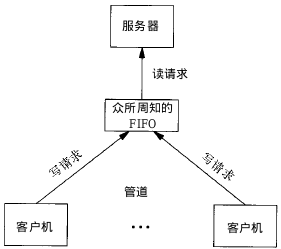
\includegraphics[scale=0.6]{fifo.png}
  \caption{FIFO管道}
  \label{fig:fifo}
\end{figure}

\subsubsection{消息队列}
消息队列,是消息的链接表,存放在内核中。一个消息队列由一个标识符(即队列ID)来标识。

消息队列拥有自己的一些特点:
\begin{itemize}
    \item 消息队列是面向记录的,其中的消息具有特定的格式以及特定的优先级。
    \item 消息队列独立于发送与接收进程。进程终止时,消息队列及其内容并不会被删除。
    \item 消息队列可以实现消息的随机查询,消息不一定要以先进先出的次序读取,也可以按消息的类型读取。
\end{itemize}

消息队列的主要原型在如下的头文件当中:
\begin{code-block}{c}
#include <sys/msg.h>
// 创建或打开消息队列:成功返回队列ID,失败返回-1
int msgget(key_t key, int flag);
// 添加消息:成功返回0,失败返回-1
int msgsnd(int msqid, const void *ptr, size_t size, int flag);
// 读取消息:成功返回消息数据的长度,失败返回-1
int msgrcv(int msqid, void *ptr, size_t size, long type,int flag);
// 控制消息队列:成功返回0,失败返回-1
int msgctl(int msqid, int cmd, struct msqid_ds *buf);
\end{code-block}

在以下两种情况下,msgget将创建一个新的消息队列:
\begin{itemize}
    \item 如果没有与键值key相对应的消息队列,并且flag中包含了IPC\_CREAT标志位。
    \item key参数为IPC\_PRIVATE
\end{itemize}

函数msgrcv在读取消息队列时,type参数有下面几种情况:
\begin{itemize}
    \item type == 0,返回队列中的第一个消息
    \item type > 0,返回队列中消息类型为 type 的第一个消息
    \item type < 0,返回队列中消息类型值小于或等于 type 绝对值的消息,如果有多个,则取类型值最小的消息
\end{itemize}

可以看出,type值非0时用于以非先进先出次序读消息。也可以把type看做优先级的权值。
下面的例子使用消息队列进行IPC,服务端程序一直在等待特定类型的消息,当收到该类型的
消息以后,发送另一种特定类型的消息作为反馈,客户端读取该反馈并打印出来。
\begin{code-block}{c}
// server.c
#include <stdio.h>
#include <stdlib.h>
#include <sys/msg.h>
#include <unistd.h>

// 用于创建一个唯一的key
#define MSG_FILE "/etc/passwd"

// 消息结构
struct msg_form {
        long mtype;
        char mtext[256];
};

int main()
{
        int msqid;
        key_t key;
        struct msg_form msg;
        // 获取key值
        // 只有server端和client端获得的key相同,server端和client端才能进行通信
        if((key = ftok(MSG_FILE,'z')) < 0)
        {
                perror("ftok error");
                exit(1);
        }

        // 打印key值
        printf("Message Queue - Server key is: %d.\n", key);

        // 创建消息队列
        if ((msqid = msgget(key, IPC_CREAT|0777)) == -1)
        {
                perror("msgget error");
                exit(1);
        }

        // 打印消息队列ID及进程ID
        printf("My msqid is: %d.\n", msqid);
        printf("My pid is: %d.\n", getpid());

        // 循环读取消息
        for(;;)
        {
                msgrcv(msqid, &msg, 256, 888, 0);// 返回类型为888的第一个消息
                printf("Server: receive msg.mtext is: %s.\n", msg.mtext);
                printf("Server: receive msg.mtype is: %d.\n", msg.mtype);

                msg.mtype = 999; // 客户端接收的消息类型
                sprintf(msg.mtext, "hello, I'm server %d", getpid());
                msgsnd(msqid, &msg, sizeof(msg.mtext), 0);
        }
        return 0;
}
\end{code-block}

而客户端的代码有区别
\begin{code-block}{c}
// client.c
#include <stdio.h>
#include <stdlib.h>
#include <sys/msg.h>
#include <unistd.h>

// 用于创建一个唯一的key
#define MSG_FILE "/etc/passwd"

// 消息结构
struct msg_form {
        long mtype;
        char mtext[256];
};

int main()
{
        int msqid;
        key_t key;
        struct msg_form msg;

        // 获取key值
        if ((key = ftok(MSG_FILE, 'z')) < 0)
        {
                perror("ftok error");
                exit(1);
        }

        // 打印key值
        printf("Message Queue - Client key is: %d.\n", key);

        // 打开消息队列
        if ((msqid = msgget(key, IPC_CREAT|0777)) == -1)
        {
                perror("msgget error");
                exit(1);
        }

        // 打印消息队列ID及进程ID
        printf("My msqid is: %d.\n", msqid);
        printf("My pid is: %d.\n", getpid());

        // 添加消息,类型为888
        msg.mtype = 888;
        sprintf(msg.mtext, "hello, I'm client %d", getpid());
        msgsnd(msqid, &msg, sizeof(msg.mtext), 0);

        // 读取类型为999的消息
        msgrcv(msqid, &msg, 256, 999, 0);
        printf("Client: receive msg.mtext is: %s.\n", msg.mtext);
        printf("Client: receive msg.mtype is: %d.\n", msg.mtype);
        return 0;
}
\end{code-block}

比较有意思的是,内核的消息队列和真正的消息队列服务器行为一致。当消息发出,没有接收者
时,依然会存在消息积压,只不过这些消息是积压在内核空间的。当接收者出现之后,这些
积压在内核空间的消息,还是会被正确投递。

\subsubsection{信号量}
信号量(semaphore)与已经介绍过的IPC结构不同,它是一个计数器。信号量用于实现进程间的互斥与同步,而不是用于存储进程间通信数据。
\begin{itemize}
    \item 信号量用于进程间同步,若要在进程间传递数据需要结合共享内存。
    \item 信号量基于操作系统的PV操作,程序对信号量的操作都是原子操作
    \item 每次对信号量的PV操作不仅限于对信号量值加1或减1,而且可以加减任意正整数。
    \item 支持信号量组。
\end{itemize}

最简单的信号量是只能取0和1的变量,这也是信号量最常见的一种形式,叫做二值信号量(Binary Semaphore)。而可以取多个正整数的信号量被称为通用信号量。
Linux下的信号量函数都是在通用的信号量数组上进行操作,而不是在一个单一的二值信号量上进行操作。实际应用时,我们每次都需要创建一个信号量集,
即使此集合只包含一个信号量。一般我们通过下面函数去创建或者打开一个信号量集。
\begin{code-block}{c}
int semget(key_t key,int nsems,int semflg);
\end{code-block}

当semflg=IPC\_CREATE时,如果当前系统中不存在此信号量集合(key值不存在),
那么semget函数完成一个信号量的创建;否则,semget函数打开这个已存在的信号量集。
当semflg=IPC\_CREATE|IPC\_EXCL时,只会完成创建,如果key值对应的信号量集合以存在,
那么直接返回错误,错误代码为EEXIST。这并不难理解,和open文件的情况类似。此函数
成功执行返回信号量集的标示符,否则为-1。

而常用的信号量函数如下:
\begin{code-block}{c}
#include <sys/sem.h>
// 创建或获取一个信号量组:若成功返回信号量集ID,失败返回-1
int semget(key_t key, int num_sems, int sem_flags);
// 对信号量组进行操作,改变信号量的值:成功返回0,失败返回-1
int semop(int semid, struct sembuf semoparray[], size_t numops);
// 控制信号量的相关信息
int semctl(int semid, int sem_num, int cmd, ...);
\end{code-block}

当semget创建新的信号量集合时,必须指定集合中信号量的个数(即num\_sems),通常为1;
如果是引用一个现有的集合,则将sems\_num指定为 0 。sembuf结构的定义如下:
\begin{code-block}{c}
struct sembuf
{
    short sem_num; // 信号量组中对应的序号,0~sem_nums-1
    short sem_op;  // 信号量值在一次操作中的改变量
    short sem_flg; // IPC_NOWAIT, SEM_UNDO
}
\end{code-block}

通过semid和sem\_num两个字段就可以确定信号量集中的指定信号量。sem\_op取不同的值就会
产生不同的操作。特别的,如果其值为0,则此时sem\_op操作的作用是测试信号量的值是否为0。
sem\_op是一次操作中的信号量的改变量,若sem\_op > 0,表示进程释放相应的资源数,将
sem\_op的值加到信号量的值上。如果有进程正在休眠等待此信号量,则唤醒他们。

若sem\_op < 0,请求sem\_op的绝对值的资源,如果相应的资源数可以满足请求,则将该信号量的值减去sem\_op的绝对值,
函数成功返回。当相应的资源数不能满足请求时,这个操作与sem\_flg有关。sem\_flg 指定IPC\_NOWAIT,则semop函数出错
返回EAGAIN。sem\_flg 没有指定IPC\_NOWAIT,则将该信号量的semncnt值加1,然后进程挂起直到下述情况发生:当相应的
资源数可以满足请求,此信号量的semncnt值减1,该信号量的值减去sem\_op的绝对值。成功返回;此信号量被删除,函数
smeop出错返回EIDRM;进程捕捉到信号,并从信号处理函数返回,此情况下将此信号量的semncnt值减1,函数semop出错
返回EINTR。

若sem\_op==0,进程阻塞直到信号量的相应值为0:当信号量已经为0,函数立即返回。如果信号量的值不为0,则依据
sem\_flg决定函数动作:sem\_flg指定IPC\_NOWAIT,则出错返回EAGAIN。sem\_flg没有指定IPC\_NOWAIT,则将该信号量的
semncnt值加1,然后进程挂起直到下述情况发生:信号量值为0,将信号量的semzcnt的值减1,函数semop成功返回;此
信号量被删除,函数smeop出错返回EIDRM;进程捕捉到信号,并从信号处理函数返回,在此情况将此信号量的semncnt值
减1,函数semop出错返回EINTR。

在semctl函数中的命令有多种,这里就说两个常用的:SETVAL:用于初始化信号量为一个已知的值。所需要的值作为联合
semun的val成员来传递。在信号量第一次使用之前需要设置信号量。IPC\_RMID:删除一个信号量集合。如果不删除信号量,
它将继续在系统中存在,即使程序已经退出,它可能在你下次运行此程序时引发问题,而且信号量是一种有限的资源。

一个简单的例子。如果不使用信号量,父进程会先于子进程输出。但是,使用信号量之后,子进程会先于父进程执行。
\begin{code-block}{c}
#include <stdio.h>
#include <stdlib.h>
#include <sys/sem.h>
#include <unistd.h>

union semun
{
        int              val; /*for SETVAL*/
        struct semid_ds *buf;
        unsigned short  *array;
};

// 初始化信号量
int init_sem(int sem_id, int value)
{
        union semun tmp;
        tmp.val = value;
        if(semctl(sem_id, 0, SETVAL, tmp) == -1)
        {
                perror("Init Semaphore Error");
                return -1;
        }
        return 0;
}

// P操作:
//    若信号量值为1,获取资源并将信号量值-1
//    若信号量值为0,进程挂起等待
int sem_p(int sem_id)
{
        struct sembuf sbuf;
        sbuf.sem_num = 0; /*序号*/
        sbuf.sem_op = -1; /*P操作*/
        sbuf.sem_flg = SEM_UNDO;

        if(semop(sem_id, &sbuf, 1) == -1)
        {
                perror("P operation Error");
                return -1;
        }
        return 0;
}

// V操作:
//    释放资源并将信号量值+1
//    如果有进程正在挂起等待,则唤醒它们
int sem_v(int sem_id)
{
        struct sembuf sbuf;
        sbuf.sem_num = 0; /*序号*/
        sbuf.sem_op = 1;  /*V操作*/
        sbuf.sem_flg = SEM_UNDO;

        if(semop(sem_id, &sbuf, 1) == -1)
        {
                perror("V operation Error");
                return -1;
        }
        return 0;
}

// 删除信号量集
int del_sem(int sem_id)
{
        union semun tmp;
        if(semctl(sem_id, 0, IPC_RMID, tmp) == -1)
        {
                perror("Delete Semaphore Error");
                return -1;
        }
        return 0;
}


int main()
{
        int sem_id;  // 信号量集ID
        key_t key;
        pid_t pid;

        // 获取key值
        if((key = ftok(".", 'z')) < 0)
        {
                perror("ftok error");
                exit(1);
        }

        // 创建信号量集,其中只有一个信号量
        if((sem_id = semget(key, 1, IPC_CREAT|0666)) == -1)
        {
                perror("semget error");
                exit(1);
        }

        // 初始化:初值设为0资源被占用
        init_sem(sem_id, 0);

        if((pid = fork()) == -1)
                perror("Fork Error");
        else if(pid == 0) /*子进程*/
        {
                //sleep(2);
                printf("Process child: pid=%d\n", getpid());
                sem_v(sem_id);  /*释放资源*/
        }
        else  /*父进程*/
        {
                sem_p(sem_id);   /*等待资源*/
                printf("Process father: pid=%d\n", getpid());
                sem_v(sem_id);   /*释放资源*/
                del_sem(sem_id); /*删除信号量集*/
        }
        return 0;
}
\end{code-block}
